\documentclass[12pt]{extarticle}
\usepackage[utf8]{inputenc}
%\usepackage{cite}
\usepackage[autolang=other,backend=biber,dateabbrev=false,sorting=none]{biblatex}
\usepackage{graphicx}
\usepackage{subcaption}
\usepackage{amsmath}
\usepackage{pdfpages}
\usepackage{listings}
\usepackage{float}
\usepackage[format=plain,
            labelfont={bf},
            textfont=it]{caption}
\lstset{
basicstyle=\fontsize{11}{13}\selectfont\ttfamily,
frame=single
}
\usepackage{hyperref}

\addbibresource{ra.bib}

\title{Software Design Descriptoon: CSM Miner}
\author{
Odysseas Karanikas\\
\texttt{odysseas.karanikas@rwth-aachen.de}
\and
Mann, Daniel\\
\texttt{daniel.mann@rwth-aachen.de}
\and
Daniel Rein\\
\texttt{drein99@outlook.de}
}

\date{May 2019}

\begin{document}


\maketitle

\section{Introduction}
\subsection{Purpose}
This document contains the complete design description of the Web Application for CSM Miner. \\
The architectural features of the system consisting of the front-end and the back-end will be explained in detail. \\
The primary audiences of this document are the software developers. 

\subsection{Scope}
As already mentioned, the system consists of two major subsystems communicating with each other. The front-end will be a Web Application where the user can upload an event log, generate a visual representation of this log and can then edit the log and generate different views. \\
The back-end will receive the event log from the Web Application, returning the generated views which are then shown in the Web Application.

\subsection{Overview of the Document}

\section{Architectural Design}

\subsection{Unit Design: Web Application}

\begin{figure}[H]
    \centering
    \begin{subfigure}[b]{0.85\textwidth}
        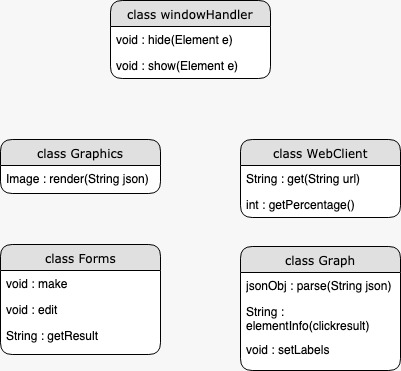
\includegraphics[width=\textwidth]{img3.jpeg}
        \label{fig:arc_1}
    \end{subfigure}
\end{figure}

\subsubsection{windowHandler}
Description: This class will be able to show and hide HTML Objects. \\ \\
Operations: \\
    void: hide(Element e) \\
    Arguments: An HTML Object \\
	Returns: Nothing returned. \\
	Description: This method will hide the HTML Element e. \\ \\
	void: show(Element e) \\
    Arguments: An HTML Object \\
	Returns: Nothing returned. \\
	Description: This method will show the HTML Element e. \\

\subsubsection{Graphics}
Description: This class will render the graphs. \\ \\
Operations: \\
    Image: render(String json) \\
    Arguments: A json file \\
	Returns: The rendered image of the graph defined in the json file. \\
	Description: This method will geneare a graph according to the json file. \\

\subsubsection{Forms}
Description: This class will handle the forms used. \\ \\
Operations: \\
    void: make() \\
    Arguments: None. \\
	Returns: Nothing returned. \\
	Description: This method will generate a form. \\ \\
	void: edit() \\
    Arguments: None. \\
	Returns: Nothing returned. \\
	Description: This method will edit the appearance of a form. \\ \\
	String: getResult() \\
    Arguments: None. \\
	Returns: A String containing the content of a form. \\
	Description: This method will return the content of a form. \\

\subsubsection{WebClient}
Description: This class will receive the data from the back-end. \\ \\
Operations: \\
    String: get(String url) \\
    Arguments: A String containing the url. \\
	Returns: Returns a json file. \\
	Description: This method will return a json file form the url as a String. \\ \\
	int: getPercentage() \\
    Arguments: None. \\
	Returns: A percentage of the download status. \\
	Description: This method will calculate the current download status and return the percentage. \\

\subsubsection{Graph}
Description: This class will represent a graph. \\ \\
Operations: \\
    jsonObj: parse(String json) \\
    Arguments: A json file. \\
	Returns: A json object. \\
	Description: This method will generate the graph according to the json file and will return a json Object. \\ \\
	String: elementInfo(clickresult) \\
    Arguments: The object the user clicked on. \\
	Returns: The information the user demands. \\
	Description: This method will return the information associated to the object the user clicked on. \\ \\
	void: setLabels() \\
    Arguments: None. \\
	Returns: Nothing returned. \\
	Description: This method will make a webRequest to edit a label in a graph. \\
	
	
\subsection{Unit Design: URLs}

\begin{figure}[H]
    \centering
    \begin{subfigure}[b]{0.35\textwidth}
        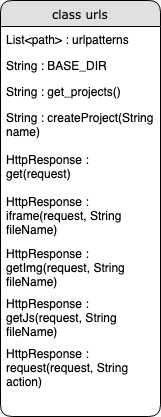
\includegraphics[width=\textwidth]{img2.jpeg}
        \label{fig:arc_1}
    \end{subfigure}
\end{figure}

\subsubsection{urls}
Description: This class will generate responses to received HttpRequests. \\ \\
Attributes:
    String BASE\textunderscore DIR \\
    Description: The String will contain the server directory.
Operations: \\
	String: get\textunderscore projects() \\
    Arguments: None. \\
	Returns: Returns a merged list as a String. \\
	Description: This method will merge all project json files and return it as a String. \\ \\
	String: createProject(String name) \\
    Arguments: The name of the project as a String. \\
	Returns: XXX. \\
	Description: This method will create a new project with a custom name. \\ \\
	HttpResponse: get(request) \\
    Arguments: A request. \\
	Returns: Returns the index.html. \\
	Description: This method will handle all the requests. \\ \\
	HttpResponse: iFrame(request, String fileName) \\
    Arguments: The request and the name of the file. \\
	Returns: Returns a html file. \\
	Description: This method will return a html file used for iframes. \\ \\
	HttpResponse: getImg(request, String fileName) \\
    Arguments: The request and the name of the file. \\
	Returns: Returns a png file. \\
	Description: This method will return a png image from the image folder. \\ \\
	HttpResponse: getJs(request, String fileName) \\
    Arguments: The request and the name of the file. \\
	Returns: Returns a js file. \\
	Description: This method will return a js file used for external resources. \\ \\
	HttpResponse: request(request, String fileName) \\
    Arguments: The request and the name of the file. \\
	Returns: Returns a json file. \\
	Description: This method will generate a json file for a request (e. g. generate Graph, labeling, etc.). \\

\section{Data Structure Design}

\subsection{Back-End}

\begin{tabular}{ | l | l | l |}
    \hline
    Field & Type & Description \\ \hline
    test & test & test \\
    \hline
\end{tabular}

\section{User Interface Design}
After the user connects to the Web Application, he is presentet with the project view where he can create a new project or load an already existing project. He can create a project by uploading a .xes file. The front-end will then generate a general view for the user to look at and interact with. \\
When the user has decided which project he wants to edit or view, the Web Application will show him or her the current views he or she has requested. At the bottom of the screen a little window displays the information for the object the user clicked on. On the top of the screen is a menu bar the user can interact with. \\
The most of the screen is the main view in which the user can interact with the graphical representation of his event log. At the right hand side there are all other available views for the user to select. The selected view from the list on the right will then change with the main view, so the user can then interact with the new selected view.


\section{Use Case Relations}

\begin{figure}[H]
    \centering
    \begin{subfigure}[b]{0.85\textwidth}
        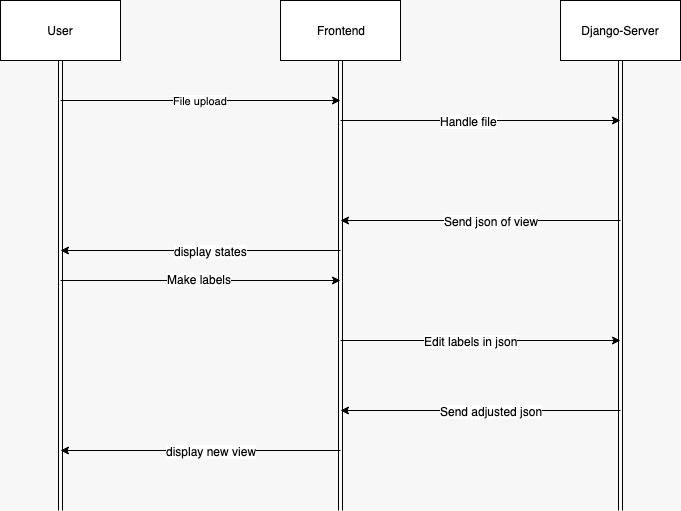
\includegraphics[width=\textwidth]{img1.jpeg}
        \label{fig:arc_1}
    \end{subfigure}
\end{figure}

\end{document}
